%************************************************
\chapter{Resultados}\label{ch:resultados}
%************************************************
\section{Búsqueda de parámetros}

La búsqueda de parámetros para los modelos de ecuaciones de Glass se realizó usando diferentes combinaciones de funciones objetivo y estrategias de búsqueda. La implementación de las rutinas se realizó en lenguaje C \citep{Kernighan1988} bajo el estándar \textsc{iso c99} publicado por \citet{c99} usando el compilador \textsc{clang} \citep{clang}. Adicionalmente, se usaron los módulos de estadística, métodos de solución de ecuaciones diferenciales ordinarias, vectores y matrices, y generación de números aleatorios de la biblioteca de funciones para cómputo científico \textsc{GNU Scientific Library (GSL) v.1.15} \citep{gslManual}.

Para la solución de ecuaciones diferenciales se utilizó el método de Euler \citeauthor{numrecipesc} \citep{numrecipesc}. También se utilizaron el método de Runge-Kutta 4,5 \citeauthor{numrecipesc} \citep{numrecipesc}, \citep{gslManual}; y el método de paso adaptativo de Adams-Bashforth \citep{gslManual}. Estos dos últimos métodos son menos sensibles a errores que el método de Euler original.

El método de Euler se implementó directamente, mientras que para el caso del método de Runge-Kutta 4,5 y del método de Adams-Bashforth se utilizó la implementación de la \textsc{GNU Scientific Library (GSL) v.1.15}. La generación de números aleatorios se realizó usando la implementación de la \textsc{GNU Scientific Library (GSL) v.1.15} del algoritmo \textsc{ranlxs2}.

Como esquema general, los programas de inferencia de parámetros consistían en proponer soluciones candidato y evaluarlas, repitiendo el proceso hasta cumplir con un criterio de paro. Una solución candidato consiste en un conjunto de parámetros propuestos de acuerdo a una estrategia de exploración del espacio de búsqueda y las trayectorias solución del problema de condiciones iniciales del sistema de ecuaciones de Glass correspondiente a dichos parámetros. La evaluación de candidatos consistió en comparar la señal original o medición experimental con la dinámica de Glass del nodo correspondiente a dicha señal o medición experimental.

\subsection{Modelo de tres nodos}

Para el modelo discreto de tres nodos, dado por:

\begin{equation}
CIS(t+\tau) = Ca^{2+}(t)
\end{equation}

\begin{equation}
Ca^{2+}(t+\tau) = CIS(t) * (Ca^{2+}ATPase(t) + 1) \% 2)
\end{equation}

\begin{equation}
Ca^{2+}ATPase(t+\tau) = Ca^{2+}(t)
\end{equation} 
\\
se implementó un modelo semicontinuo con las siguientes ecuaciones de Glass:
\begin{equation}
\frac{dCIS}{dt} = \alpha_{CIS} [F_{CIS}(\widehat{Ca^{2+}}) - CIS]
\end{equation}

\begin{equation}
\frac{dCa^{2+}}{dt} = \alpha_{Ca^{2+}} [F_{Ca^{2+}}(\widehat{CIS}, \widehat{Ca^{2+}ATPase}) - Ca^{2+}]
\end{equation}

\begin{equation}
\frac{dCa^{2+}ATPase}{dt} = \alpha_{Ca^{2+}ATPase} [F_{Ca^{2+}ATPase}(\widehat{Ca^{2+}}) - Ca^{2+}ATPase)]
\end{equation} 
\\
donde
$$\widehat{CIS} = H(CIS - \theta_{CIS})$$
\\
$$\widehat{Ca^{2+}} = H(Ca^{2+} - \theta_{Ca^{2+}})$$
\\
$$\widehat{Ca^{2+}ATPase} = H(Ca^{2+}ATPase - \theta_{Ca^{2+}ATPase})$$
\\
corresponden a los valores discretizados de las variables continuas $CIS$, $Ca^{2+}$ y $Ca^{2+}ATPase$, respectivamente. Es necesario discretizar el valor de estas variables pues hay que recordar que $F_{CIS}$, $F_{Ca^{2+}}$ y $F_{Ca^{2+}ATPase}$ son funciones cuyos argumentos son valores discretos.

Como caso de ejemplo de estimación de parámetros en un problema de transformación de un modelo discreto a un modelo semicontinuo, se resolvió mediante el método de Euler el sistema de ecuaciones de Glass de la red de 3 nodos con parámetros $\alpha_{CIS} = \alpha_{Ca^{2+}} =  \alpha_{Ca^{2+}ATPase} = 1$, umbrales de activación $\theta_{CIS} = 0.3$, $\theta_{Ca^{2+}} = 0.7$ y $\theta_{Ca^{2+}APTase} = 0.8$, y $CIS = 1$, $Ca^{2+} = 0$, $Ca^{2+}ATPase = 0$ como condiciones iniciales. El objetivo consistió en encontrar mediante un procedimiento de búsqueda el conjunto de parámetros tales que la dinámica de Glass correspondiente al $Ca^{2+}ATPase$ fuera lo más similar posible a la solución conocida para los parámetros antes mencionados. Esta solución conocida se tomó como una señal artificial, que se muestra en la figura \ref{fig:signal3nodos}.

\begin{figure}[hbt]
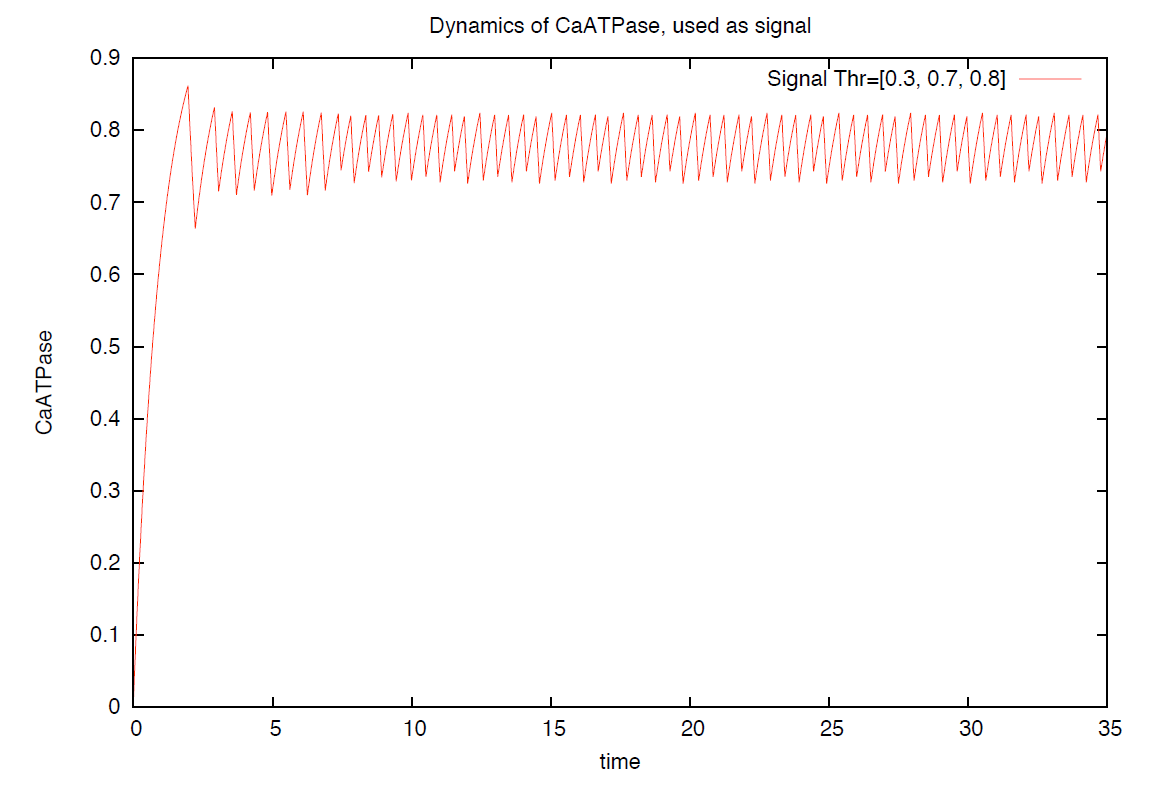
\includegraphics[width=0.9\linewidth]{gfx/original3Nodos}
\caption[Dinámica original $Ca^{2+}ATPase$]{Dinámica original de $Ca^{2+}ATPase$ de las ecucaciones de Glass con parámetros $\alpha_{CIS} = \alpha_{Ca^{2+}} =  \alpha_{Ca^{2+}ATPase} = 1$, umbrales de activación $\theta_{CIS} = 0.3$, $\theta_{Ca^{2+}} = 0.7$ y $\theta_{Ca^{2+}APTase} = 0.8$, y $CIS = 1$, $Ca^{2+} = 0$, $Ca^{2+}ATPase = 0$ como condiciones iniciales.}\label{fig:signal3nodos}
\end{figure}

Se eligió búsqueda aleatoria como estrategia de exploración del espacio de búsqueda, mientras que la función objetivo consistió en minimizar $f_{SI}(X,Y) = 1 -SI(X,Y)$ con $X$ la señal original y $Y$ los datos de la dinámica de Glass del nodo $Ca^{2+}ATPase$ de cada uno de los candidatos propuestos por el algoritmo de búsqueda.

\begin{figure}[hbt]
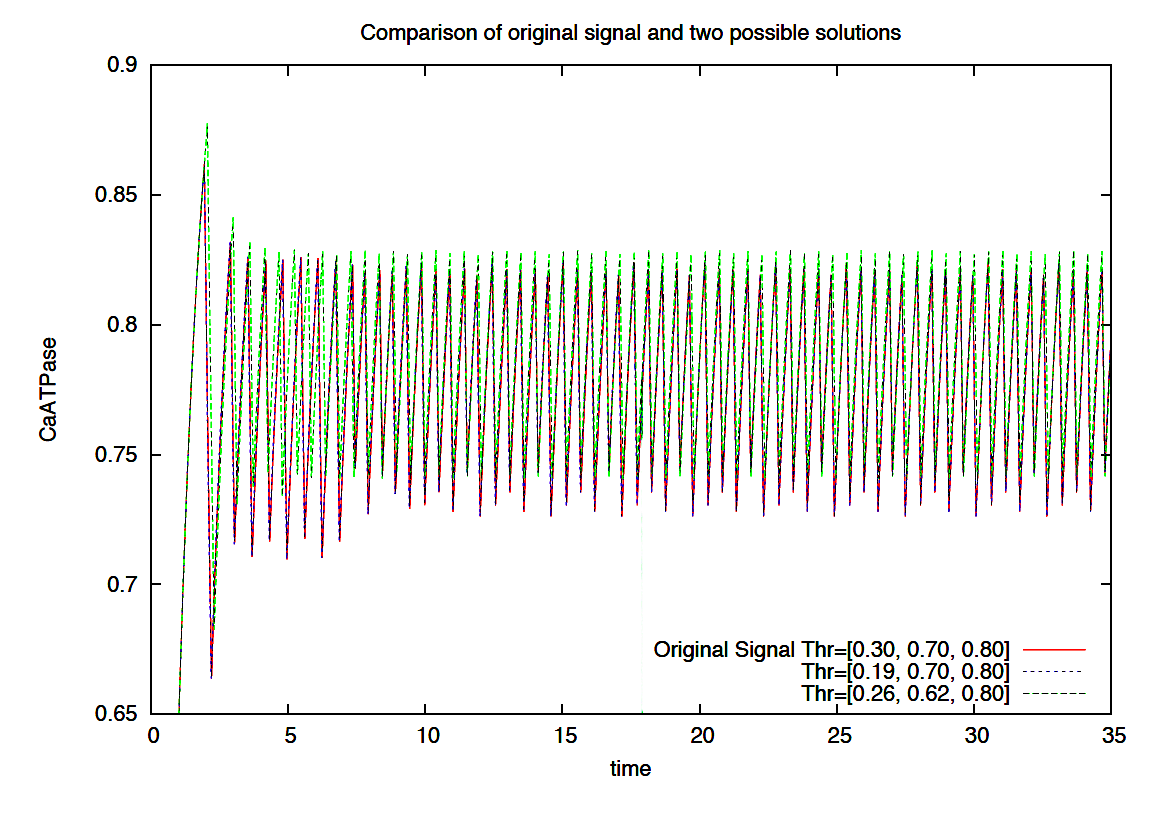
\includegraphics[width=0.9\linewidth]{gfx/comparacion3Nodos}
\caption[Dinámicas original y estimada $Ca^{2+}ATPase$]{Dinámicas original y estimada de $Ca^{2+}ATPase$ de la red de 3 nodos. En rojo la señal original, verde y azul representan dos distintas ejecuciones del programa de búsqueda.}\label{fig:resultadoChido3Nodos}
\end{figure}

En este caso, fue posible recuperar el valor de los tres parámetros en varias ejecuciones del programa de búsqueda. La figura \ref{fig:resultadoChido3Nodos} muestra la dinámica original y el resultado obtenido con dos ejecuciones distintas del programa de busqueda.

Se probó realizar la estimación de parámetros para el mismo sistema usando una versión de algoritmos genéticos adaptada a problemas con variables continuas con los parámetros recomendados por omision, tal como se refiere en \citeauthor{Haupt1998} \citep{Haupt1998}. En este caso fue posible recuperar el valor del parámetro de umbral para $Ca^{2+}ATPase$, si bien con una precisión menor.
% Después tal vez sea bueno agregar los resultados a un apéndice.

Cabe mencionar que a pesar de que este caso de ejemplo no está relacionado en un sentido bioquímico con la red de señalización de speract, sí lo está en términos de ser un modelo discreto que se quiere reescribir como semicontinuo. Además, para la estimación de parámetros se usó un solo tipo de señal o ``medición experimental'' contra la cual comparar la dinámica de cada uno de los candidatos, situación que se presentó también en la red de señalización, donde solo se cuenta con un único tipo de mediciones para tiempos largos. La experiencia ganada con este caso de ejemplo sirvió como base para abordar la estimación de parámetros del modelo semicontinuo de la vía de señalización de speract.

\subsection{Modelo de la red de señalización}

El modelo semicontinuo de la vía de señalización de speract se implementó planteando ecuaciones de Glass cuyo valor depende de un conjunto de funciones discretas, estas últimas basadas en el modelo de \citeauthor{Espinal2011} \citep{Espinal2011}. La implementación en lenguaje C de dichas funciones discretas se muestran en el apéndice \ref{ch:appendix}. A modo de ejemplo, puede considerarse la ecuación de Glass para cGMP. La tabla de verdad de la función discreta se muestra en la tabla \ref{tab:tabla_cGMP}, y la ecuación de Glass correspondiente en la ecuación \ref{eqn:glasscGMP}.

\begin{table}[hb]
    \myfloatalign
  \begin{tabularx}{\textwidth}{cccc} \toprule
    \tableheadline{GC(t)} & \tableheadline{PDE(t)} & \tableheadline{cGMP(t)} & \tableheadline{cGMP(t+1)} \\
	\midrule
	0 &	0 & 0 &	0 \\
	0 & 0 & 1 & 1 \\
	0 & 1 & 0 & 0 \\
	0 & 1 & 1 & 0 \\
	1 & 0 & 0 & 1 \\
	1 & 0 & 1 & 1 \\
	1 & 1 & 0 & 0 \\
	1 & 1 & 1 & 0 \\
    \bottomrule
  \end{tabularx}
  \caption[Tabla de regulación de cGMP]{Tabla de regulación de cGMP}
  \label{tab:tabla_cGMP}
\end{table}

Y la ecuación de Glass correspondiente es:

\begin{equation}\label{eqn:glasscGMP}
\frac{dcGMP}{dt} = \alpha_{cGMP} [F_{cGMP}(\widehat{GC}, \widehat{PDE}, \widehat{cGMP}) - cGMP]
\end{equation}
\\
donde
$$\widehat{GC} = H(GC - \theta_{GC})$$ $$\widehat{PDE} = H(PDE - \theta_{PDE})$$ y $$\widehat{cGMP} = H(cGMP - \theta_{cGMP})$$
\\
son los valores discretizados de las variables continuas $GC$, $PDE$ y $cGMP$, respectivamente.

El problema de estimación de parámetros en este caso consiste en ajustar el valor de 26 parámetros de umbral $\theta_i$ (22 para los nodos binarios y 4 extras para los nodos que tienen un valor terciario), en el caso de un sistema sincronizado donde todos los parámetros $\alpha_i=x$, $x \in [0,T_{max}]$, donde $T_{max}$ es el tiempo característico más grande del sistema. 

Un problema similar, si bien más complicado, es permitir que cada $\alpha_i$ tome un valor distinto de los demás $\alpha_i$, es decir, un problema asíncrono. El problema asíncrono añade la necesidad de estimar 22 parámetros extra, uno para cada componente del sistema.

Como una primera aproximación al problema, se consideró el problema sincronizado, estableciendo $\alpha_i = 1.0\ \forall i$, de modo que solo se debió estimar el valor de los 26 parámetros de umbral. Las condiciones iniciales se fijaron tales que el valor inicial para el potencial de membrana $V = 1.0$, los canales $HVA=LVA=1.0$, $dCA = 0.9$ y el resto con valor $0.2$. Al discretizar estos valores, se tiene una condición inicial muy similar a la del organismo silvestre según el modelo discreto antecedente de este trabajo. 

En vista de que aun para el problema sincronizado el espacio de parámetros es mayor que el del problema de 3 nodos presentado en la sección anterior, y de que los algoritmos genéticos no presentaron una mejora con respecto a la búsqueda aleatoria en el mismo problema, se buscó otro método de exploración del espacio de búsqueda. A este respecto, \citeauthor{BangaMoles2003} \citep{BangaMoles2003} muestran que para problemas de estimación de parámetros en redes de señalización bioquímica los métodos con mejores resultados son aquellos basados en estrategias evolutivas. En especial algunos como Evolución Diferencial resultan aún mejores que los algoritmos genéticos.

Para la búsqueda de parámetros de la vía de señalización de speract se usó entonces Evolución Diferencial como estrategia de búsqueda (y evaluación de candidatos), usando los parámetros recomendados en la literatura \citeauthor{Storn1997}  \citep{Storn1997}. Para comparar la dinámica del nodo de $Ca^{2+}$, (denotado en el modelo como $dCa$) de cada modelo planteado con las mediciones experimentales de fluorescencia de $Ca^{2+}$, se buscó minimizar $f_{Pearson}(X,Y) = 1-r_{X,Y}$, donde $X$ son los datos experimentales y $Y$ son los datos de la dinámica del nodo de calcio del modelo. 

Los sistemas de ecuaciones de Glass se resolvieron mediante el método de Euler. Para algunas dinámicas elegidas por el algoritmo de Evolución Diferencial, se verificó la solución usando el método de Adams-Bashforth. No se encontraron diferencias significativas entre las soluciones de uno y otro métodos.

Se logró ajustar la dinámica del nodo de $Ca^{2+}$ de acuerdo a mediciones experimentales, como se muestra en la figura \ref{fig:glassChido}. 

\begin{figure}[h]
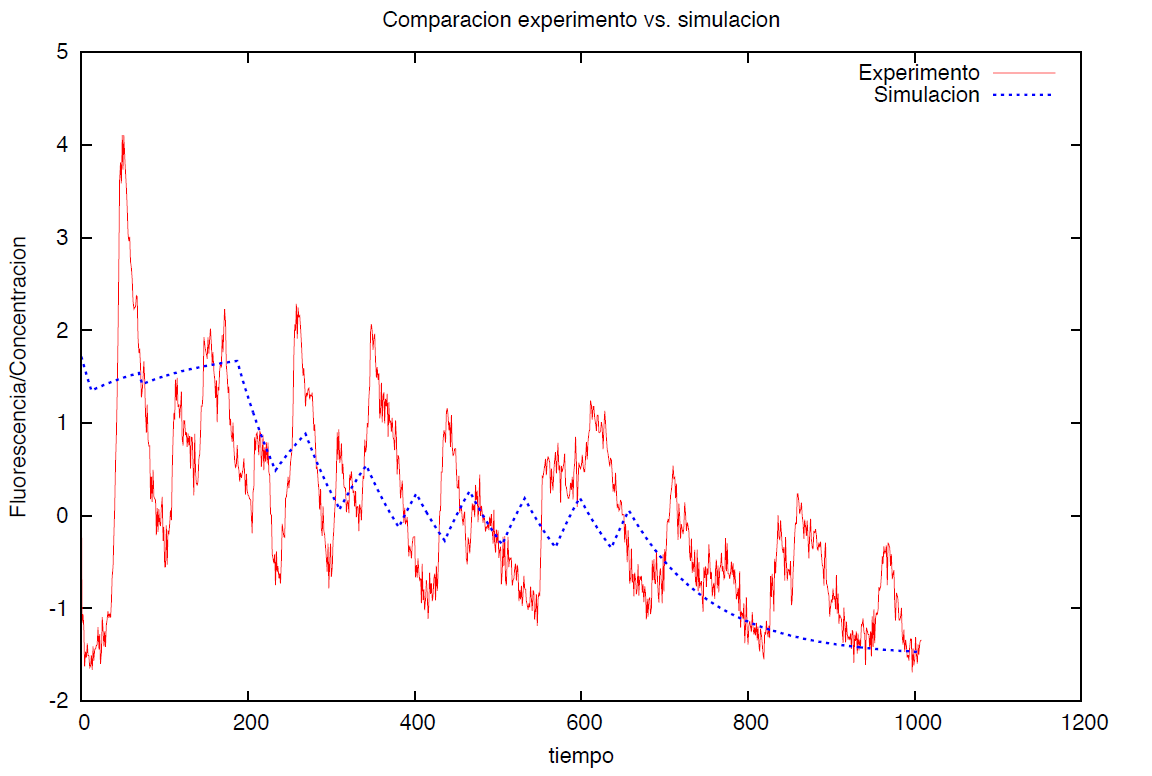
\includegraphics[width=0.9\linewidth]{gfx/glassChido}
\caption[Dinámica del nodo de $Ca^{2+}$ del modelo y medición experimental de $Ca^{2+}$]{Dinámica del nodo de $Ca^{2+}$ del modelo y medición experimental de $Ca^{2+}$. En rojo la medición experimental, en azul el ajuste usando la función objetivo basada en la correlación de Pearson. Para efectos de comparación, las series se normalizaron de manera que tuvieran promedio $0$ y varianza $1$.}\label{fig:glassChido}
\end{figure}

A pesar de lo alentador de este resultado, el comportamiento dinámico de otros nodos aún necesita mayor revisión. Por ejemplo, el nodo correspondiente al potencial de membrana $V$ debería de disminuir su valor al inicio de la dinámica para luego aumentarlo. Sin embargo, el potencial aumenta al principio y disminuye posteriormente. Este comportamiento es imposible en la realidad, ya que al haber un aumento de $[Ca^{2+}]_i$ el potencial deberia disminuir. Véase la figura \ref{fig:glassChafa}.

\begin{figure}[h]
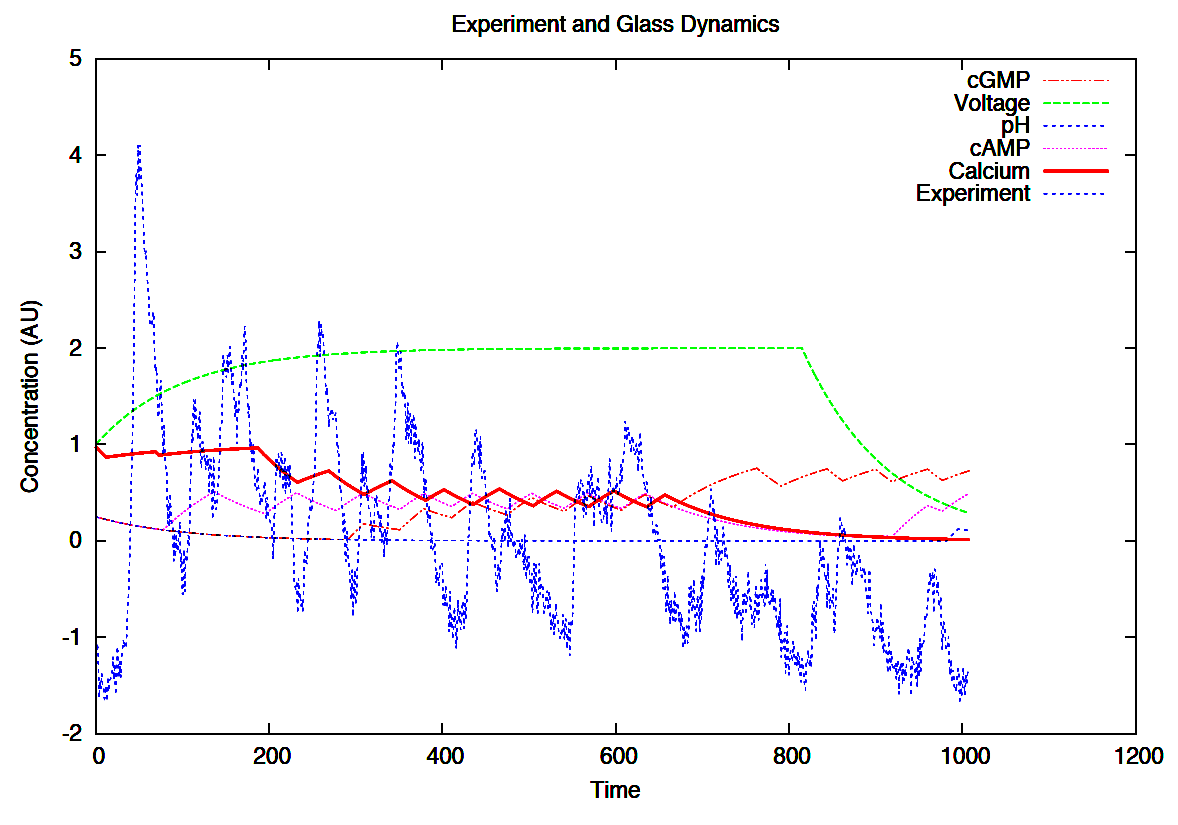
\includegraphics[width=0.9\linewidth]{gfx/glassChafa}
\caption[Dinámica de $Ca^{2+}$, $V$ y otros componentes del modelo, y medición experimental de $Ca^{2+}$]{Dinámica del nodo de $Ca^{2+}$, $V$ y otros componentes del modelo, y medición experimental de $Ca^{2+}$. En este caso en azul punteado se muestra la medición expetimental, en rojo el nodo de $Ca^{2+}$ del modelo y en verde el nodo que representa al potencial de membrana en el modelo. Nótese que se trata de una ejecución del algoritmo de búsqueda distinta a la de la figura \ref{fig:glassChido}. Para efectos de comparación, las series se normalizaron de manera que tuvieran promedio $0$ y varianza $1$.}\label{fig:glassChafa}
\end{figure}

Varias ejecuciones del algoritmo de evolución diferencial, diferentes parámetros para el mismo algoritmo y funciones objetivo distintas, es decir, usando error cuadrático medio \textsc{mse} o el índice de pendiente \textsc{(si)} arrojaron resultados similares.












































